\documentclass[12pt]{article}
\usepackage{amsbsy,amssymb,latexsym,amsfonts,amsmath}
\usepackage{graphicx,color,hyperref,braket}
\usepackage{tikz}
\usetikzlibrary{intersections, calc, arrows.meta}

\begin{document}

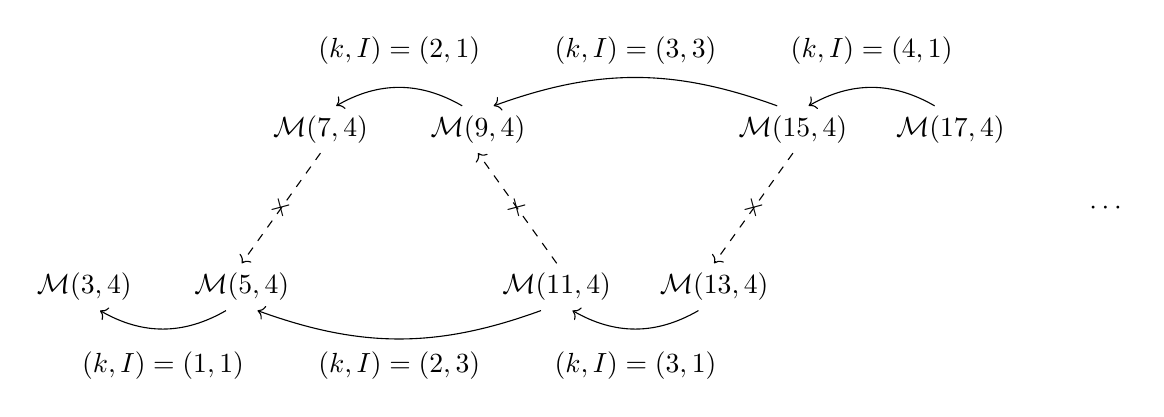
\begin{tikzpicture}
\draw(0, 0)node{$\mathcal{M}(3, 4)$};
\draw(2, 0)node{$\mathcal{M}(5, 4)$};
\draw(3, 2)node{$\mathcal{M}(7, 4)$};
\draw(5, 2)node{$\mathcal{M}(9, 4)$};
\draw(6, 0)node{$\mathcal{M}(11, 4)$};
\draw(8, 0)node{$\mathcal{M}(13, 4)$};
\draw(9, 2)node{$\mathcal{M}(15, 4)$};
\draw(11, 2)node{$\mathcal{M}(17, 4)$};
\draw[dashed, ->](3, 1.7)--(2, 0.3);
\draw(2.5, 1)node{\rotatebox{60}{$\times$}};
\draw[dashed, ->](6, 0.3)--(5, 1.7);
\draw(5.5, 1)node{\rotatebox{60}{$\times$}};
\draw[dashed, ->](9, 1.7)--(8, 0.3);
\draw(8.5, 1)node{\rotatebox{60}{$\times$}};
\draw[->](1.8, -0.3) to [out = 210, in = -30] (0.2, -0.3);
\draw(1, -1)node{$(k, I) = (1, 1)$};
\draw[->](7.8, -0.3) to [out = 210, in = -30] (6.2, -0.3);
\draw(7, -1)node{$(k, I) = (3, 1)$};
\draw[->](5.8, -0.3) to [out = 200, in = -20] (2.2, -0.3);
\draw(4, -1)node{$(k, I) = (2, 3)$};
\draw[->](4.8, 2.3) to [out = 150, in = 30] (3.2, 2.3);
\draw(4, 3)node{$(k, I) = (2, 1)$};
\draw[->](10.8, 2.3) to [out = 150, in = 30] (9.2, 2.3);
\draw(10, 3)node{$(k, I) = (4, 1)$};
\draw[->](8.8, 2.3) to [out = 160, in = 20] (5.2, 2.3);
\draw(7, 3)node{$(k, I) = (3, 3)$};
\draw(13, 1)node{$\cdots$};
\end{tikzpicture}

\end{document}